
%%%%%%%%%%%%%%%%%%%%%%%%%%%%%%%%%%%%%%%%%%%%%%%%%%%%%%%%%%%%%%%%%%%%%
%% This is a (brief) model paper using the achemso class
%% The document class accepts keyval options, which should include
%% the target journal and optionally the manuscript type.
%%%%%%%%%%%%%%%%%%%%%%%%%%%%%%%%%%%%%%%%%%%%%%%%%%%%%%%%%%%%%%%%%%%%%
\documentclass[journal=jpccck,manuscript=article]{achemso}

%%%%%%%%%%%%%%%%%%%%%%%%%%%%%%%%%%%%%%%%%%%%%%%%%%%%%%%%%%%%%%%%%%%%%
%% Place any additional packages needed here.  Only include packages
%% which are essential, to avoid problems later. Do NOT use any
%% packages which require e-TeX (for example etoolbox): the e-TeX
%% extensions are not currently available on the ACS conversion
%% servers.
%%%%%%%%%%%%%%%%%%%%%%%%%%%%%%%%%%%%%%%%%%%%%%%%%%%%%%%%%%%%%%%%%%%%%
\usepackage[version=3]{mhchem} % Formula subscripts using \ce{}
\usepackage[T1]{fontenc}       % Use modern font encodings
\usepackage{graphicx}
\usepackage{amsmath}
\usepackage{xcolor}
\usepackage{wrapfig}
%%%%%%%%%%%%%%%%%%%%%%%%%%%%%%%%%%%%%%%%%%%%%%%%%%%%%%%%%%%%%%%%%%%%%
%% If issues arise when submitting your manuscript, you may want to
%% un-comment the next line.  This provides information on the
%% version of every file you have used.
%%%%%%%%%%%%%%%%%%%%%%%%%%%%%%%%%%%%%%%%%%%%%%%%%%%%%%%%%%%%%%%%%%%%%
%%\listfiles

%%%%%%%%%%%%%%%%%%%%%%%%%%%%%%%%%%%%%%%%%%%%%%%%%%%%%%%%%%%%%%%%%%%%%
%% Place any additional macros here.  Please use \newcommand* where
%% possible, and avoid layout-changing macros (which are not used
%% when typesetting).
%%%%%%%%%%%%%%%%%%%%%%%%%%%%%%%%%%%%%%%%%%%%%%%%%%%%%%%%%%%%%%%%%%%%%
\newcommand*\mycommand[1]{\texttt{\emph{#1}}}

%%%%%%%%%%%%%%%%%%%%%%%%%%%%%%%%%%%%%%%%%%%%%%%%%%%%%%%%%%%%%%%%%%%%%
%% Meta-data block
%% ---------------
%% Each author should be given as a separate \author command.
%%
%% Corresponding authors should have an e-mail given after the author
%% name as an \email command. Phone and fax numbers can be given
%% using \phone and \fax, respectively; this information is optional.
%%
%% The affiliation of authors is given after the authors; each
%% \affiliation command applies to all preceding authors not already
%% assigned an affiliation.
%%
%% The affiliation takes an option argument for the short name.  This
%% will typically be something like "University of Somewhere".
%%
%% The \altaffiliation macro should be used for new address, etc.
%% On the other hand, \alsoaffiliation is used on a per author basis
%% when authors are associated with multiple institutions.
%%%%%%%%%%%%%%%%%%%%%%%%%%%%%%%%%%%%%%%%%%%%%%%%%%%%%%%%%%%%%%%%%%%%%
\author{Nicholas P. Montoni}
\author{Steven C. Quillin}
\author{Charles Cherqui}
\affiliation[Department of Chemistry, University of Washington]
{Department of Chemistry, University of Washington, Seattle, WA 98195}
\author{Niket Thakkar}
\affiliation[Department of Applied Mathematics, University of Washington]
{Department of Applied Mathematics, University of Washington, Seattle, WA 98195}
\author{David J. Masiello}
\affiliation[Department of Chemistry, University of Washington]
{Department of Chemistry, University of Washington, Seattle, WA 98195}
\alsoaffiliation[Department of Applied Mathematics, University of Washington]
{Department of Applied Mathematics, University of Washington, Seattle, WA 98195}
\email{masiello@chem.washington.edu}

%%%%%%%%%%%%%%%%%%%%%%%%%%%%%%%%%%%%%%%%%%%%%%%%%%%%%%%%%%%%%%%%%%%%%
%% The document title should be given as usual. Some journals require
%% a running title from the author: this should be supplied as an
%% optional argument to \title.
%%%%%%%%%%%%%%%%%%%%%%%%%%%%%%%%%%%%%%%%%%%%%%%%%%%%%%%%%%%%%%%%%%%%%
\title[]
    {Understanding Retardation Effects on the Energy Ordering of Magnetic Plasmons}
%%%%%%%%%%%%%%%%%%%%%%%%%%%%%%%%%%%%%%%%%%%%%%%%%%%%%%%%%%%%%%%%%%%%%
%% Some journals require a list of abbreviations or keywords to be
%% supplied. These should be set up here, and will be printed after
%% the title and author information, if needed.
%%%%%%%%%%%%%%%%%%%%%%%%%%%%%%%%%%%%%%%%%%%%%%%%%%%%%%%%%%%%%%%%%%%%%
\abbreviations{MNP, LSPR, EELS}
\keywords{plasmon, hybridization, magnetic, retardation}

%%%%%%%%%%%%%%%%%%%%%%%%%%%%%%%%%%%%%%%%%%%%%%%%%%%%%%%%%%%%%%%%%%%%%
%% The manuscript does not need to include \maketitle, which is
%% executed automatically.
%%%%%%%%%%%%%%%%%%%%%%%%%%%%%%%%%%%%%%%%%%%%%%%%%%%%%%%%%%%%%%%%%%%%%
\begin{document}

%%%%%%%%%%%%%%%%%%%%%%%%%%%%%%%%%%%%%%%%%%%%%%%%%%%%%%%%%%%%%%%%%%%%%
%% The "tocentry" environment can be used to create an entry for the
%% graphical table of contents. It is given here as some journals
%% require that it is printed as part of the abstract page. It will
%% be automatically moved as appropriate.
%%%%%%%%%%%%%%%%%%%%%%%%%%%%%%%%%%%%%%%%%%%%%%%%%%%%%%%%%%%%%%%%%%%%%
\begin{tocentry}

Some journals require a graphical entry for the Table of Contents.
This should be laid out ``print ready'' so that the sizing of the
text is correct.

Inside the \texttt{tocentry} environment, the font used is Helvetica
8\,pt, as required by \emph{Journal of the American Chemical
Society}.

The surrounding frame is 9\,cm by 3.5\,cm, which is the maximum
permitted for  \emph{Journal of the American Chemical Society}
graphical table of content entries. The box will not resize if the
content is too big: instead it will overflow the edge of the box.

This box and the associated title will always be printed on a
separate page at the end of the document.

\end{tocentry}

%%%%%%%%%%%%%%%%%%%%%%%%%%%%%%%%%%%%%%%%%%%%%%%%%%%%%%%%%%%%%%%%%%%%%
%% The abstract environment will automatically gobble the contents
%% if an abstract is not used by the target journal.
%%%%%%%%%%%%%%%%%%%%%%%%%%%%%%%%%%%%%%%%%%%%%%%%%%%%%%%%%%%%%%%%%%%%%
\begin{abstract}
Magnetic plasmons, the collective response of cyclic arrangements of electric plasmon-supporting metal nanoparticles, have been of recent theoretical and experimental interest. As magnetic-plasmon-supporting aggregates are often large (hundreds of nanometers to microns in size), information takes time to propagate across such nanostructures. As a result, they are not well-described in the quasistatic limit with plasmon hybridization theory. In this Letter it is shown that for small magnetic oligomers the quasistatic approximation is sufficient, but, as the systems grow in size, retardation effects must be considered. The quasistatic tight-binding model can be manipulated to include retardation effects by utilizing the full electric field of a dipole. This fully retarded tight-binding model accurately predicts the energy-ordering of magnetic plasmon modes in agreement with full-wave simulations.
\end{abstract}

%%%%%%%%%%%%%%%%%%%%%%%%%%%%%%%%%%%%%%%%%%%%%%%%%%%%%%%%%%%%%%%%%%%%%
%% Start the main part of the manuscript here.
%%%%%%%%%%%%%%%%%%%%%%%%%%%%%%%%%%%%%%%%%%%%%%%%%%%%%%%%%%%%%%%%%%%%%
When an electric field is incident upon a metal surface, the metal imperfectly screens the electric field, allowing penetration up to a distance known as the skin depth. When the spatial extent of a metal nanoparticle (MNP) is on the order of the skin depth, the external electric field penetrates the entire particle and forces the conduction electrons to collect at the surface.\cite{KREIBIG1985}. Releasing the force causes the electrons to oscillate collectively and coherently about their equilibrium configuration until the energy dissipates. The conduction electrons oscillate at a characteristic frequency that depends on the material and morphology of the MNP. When resonantly driven by an oscillating electric field, a localized surface plasmon resonance (LSPR), or simply a plasmon, is excited, with the lowest energy excitation being dipolar in character.

Bringing two MNPs together causes their individual plasmons to hybridize, producing a new set of plasmonic modes\cite{Lucas1976,ARAVIND1981,Xu1995,Mischenko1995}. Plasmon hybridization theory is applied to aggregates of MNPs and explains their collective behavior within the quasistatic limit in which the speed of light is taken to be infinite\cite{NordHal2003,NordProdan2004,Oubre2004,Gomez2009}. Recently, retardation effects on plasmon hybridization have been the focus of study for large particles\cite{Abajo2008,Gu2010} as well as dimers\cite{vonPlessen2007,Rechbacher2003,Kottman2001}, and 2-D arrays\cite{Schatz2003,Royer2005,Chumanov2010} of nanoparticles. Specific arrangements of nanoparticles in 2-D arrays, such as three or more nanoparticles arranged on the vertices of a regular polygon, support a collective mode in which all of the dipole plasmons are oriented head-to-tail, as demonstrated in Figure~\ref{fig1}. This generates a fictitious, oscillating current loop resulting in an oscillating magnetic dipole moment in the center of the ring\cite{Alu2006,Alu2008,Liu2011,Nord2006,Cherqui2014}. These so-called magnetic plasmons are the lowest-energy collective modes of the oligomers and couple to and enhance the magnetic field of incident light\cite{Shalaev2007,Qian2015,Nord2007}, offering a route to applications such as solar cell enhancement\cite{Graydon2011,Alu2014solar,Le2015solar}, biosensing and detection\cite{Zia2010trans,Noginova2008trans,Wang:13,Fan2015,Wei2015,Shvets2012,Altug2012bio,Nord2011fano}, and information storage and propagation\cite{Zhang2006,NordHal2011,NordHal2012}. The rich plasmonic modes of magnetic-plasmon-supporting systems are well-described using plasmon hybridization theory, but when in the quasistatic limit, the energy-ordering of the modes is not.

Plasmon hybridization theory treats LSPRs as point dipoles centered on their associated nanoparticles that interact through dipole-dipole coupling. In the quasistatic limit, these dipoles couple only through time-independent, electric near-field interactions\cite{jackson_classical_1999}:

\begin{equation}
  U_{\textrm{qs}} = -\textbf{p}_2 \cdot \textbf{E}_{\textrm{qs},1} = -\left[\frac{3(\textbf{p}_2 \cdot \hat{\textbf{r}}) (\hat{\textbf{r}} \cdot \textbf{p}_1) - \textbf{p}_2 \cdot \textbf{p}_1}{r^3}\right] = -\textbf{p}_2 \cdot \boldsymbol{\Lambda}_{\textrm{qs}} \cdot \textbf{p}_1, \label{eqn1}
  \end{equation}

where, $\textbf{p}_i$ is the dipole moment of each plasmon, $\textbf{E}_{\textrm{qs}}$ is the near-electric field in the quasistatic limit, and $r$ is the distance between dipoles with associated unit vector $\hat{\textbf{r}}$.

When the distance between nanoparticles becomes large, this approximation breaks down and intermediate- and far-field effects must be considered, as well as the time-delay effects in the near-field\cite{jackson_classical_1999}:

\begin{equation}
  U_{\textrm{NF}} = U_{\textrm{qs}}\, \cos\left(\frac{\omega r}{c}\right)=-\textbf{p}_2 \cdot \boldsymbol{\Lambda}_{\textrm{NF}} \cdot \textbf{p}_1 ;\label{near}
  \end{equation}

\begin{equation}
  U_{\textrm{IF}} = -\textbf{p}_2 \cdot \textbf{E}_{\textrm{IF},1} = \frac{\omega}{c}\left[\frac{3(\textbf{p}_2 \cdot \hat{\textbf{r}})( \hat{\textbf{r}} \cdot \textbf{p}_1) - \textbf{p}_2 \cdot \textbf{p}_1}{r^2}\right]\,\sin\left(\frac{\omega r}{c}\right)=-\textbf{p}_2 \cdot \boldsymbol{\Lambda}_{\textrm{IF}} \cdot \textbf{p}_1 ; \label{eqn2}
\end{equation}

\begin{equation}
  U_{\textrm{FF}} = -\textbf{p}_2 \cdot \textbf{E}_{\textrm{FF},1} = \frac{\omega^2}{c^2}\left[\frac{\textbf{p}_2 \cdot \textbf{p}_1 -(\textbf{p}_2 \cdot \hat{\textbf{r}}) (\hat{\textbf{r}} \cdot \textbf{p}_1)}{r}\right]\,\cos\left(\frac{\omega r}{c}\right)=-\textbf{p}_2 \cdot \boldsymbol{\Lambda}_{\textrm{FF}} \cdot \textbf{p}_1; \label{eqn3}
\end{equation}

where $\omega$ refers to the resonance frequency of a particular plasmonic mode. The aim of this Letter is to incorporate the fully retarded electric field into plasmon hybridization theory and extend studies of retardation effects to magnetic plasmon oligomers. Specifically, systems of metal nanoparticles arranged in shapes analogous to benzene and naphthalene are explored\cite{Cherqui2014}. The benzene-like ring, comprising six nanoparticles as diagrammed in Figure~\ref{fig1}D, is denoted the magnetic monomer and forms the basic magnetic unit cell. The naphthalene-like ring comprises ten nanoparticles and is constructed with two monomers sharing two central nanoparticles; consequently, it is denoted the magnetic dimer and it is diagrammed in Figure~\ref{fig1}. Through theory and simulation, it will be shown that the magnetic eigenmodes of large dimer systems can be obtained through quasistatic plasmon hybridization theory, but that their energy-ordering requires consideration of retardation effects.

%\begin{wrapfigure}
\begin{figure}
  \begin{center}
  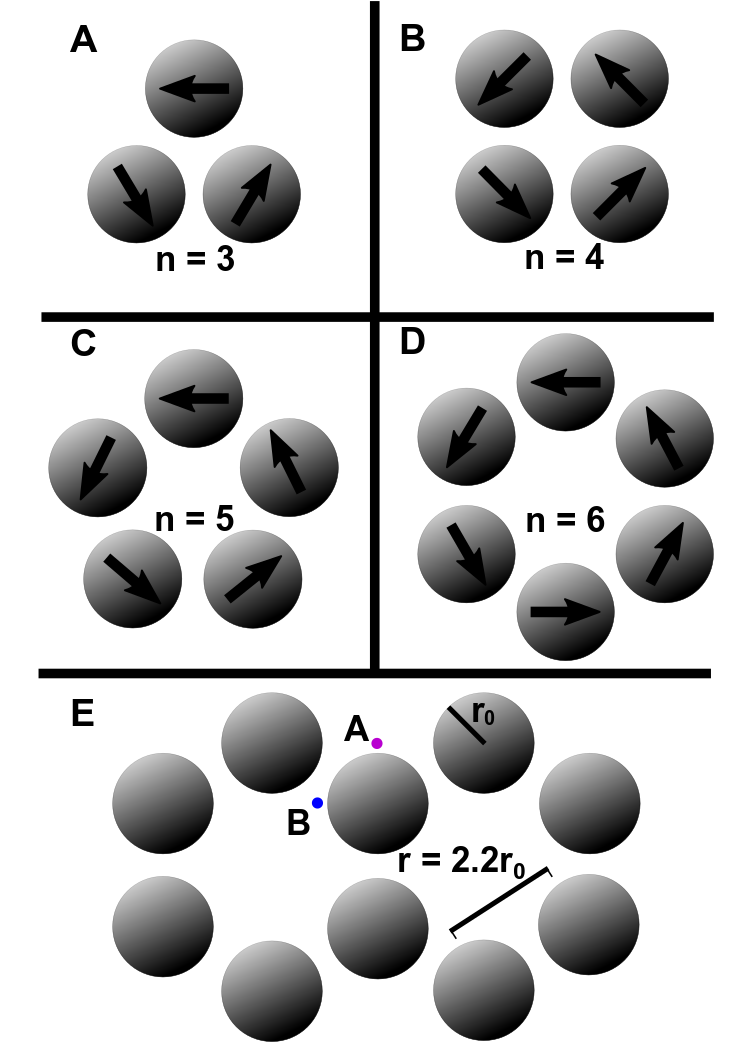
\includegraphics[trim = 0.5in 0 0.3in 0,clip=true,scale=0.4]{all_the_diagrams.png}
  \caption{Four examples of magnetic oligomer rings and their lowest-energy collective mode exhibiting a magnetic dipole moment. Note that each dipole is oriented ``tip-to-tail.'' This is similar to the lowest-energy mode of aromatic rings as diagrammed in various Frost diagrams in which the carbon ring has no nodes in its electron density. Panel E diagrams the magnetic oligomer dimer system, constructed from two of the magnetic oligomers in panel D. $r_0$ is the radius of each sphere and $r=2.2r_0$ is the center-to-center separation distance between spheres. To study this system with EELS, placing the electron beam at the purple dot (A) selectively excites the north-south mode and placing the beam at the blue dot (B) selectively excites the north-north mode.}
  \label{fig1}
  \end{center}
\end{figure}
%\end{wrapfigure}

For the magnetic dimer, only the two planar dipoles per particle are considered in the tight binding model, yielding a total of twenty. The dipoles are mapped onto a set of harmonic oscillators and are described by the following Hamiltonian:

\begin{equation}
  H = \sum_{i=1}^{n}\left[\frac{1}{2m_{sp,i}}\textbf{P}_{i}^{2}+\frac{1}{2}m_{sp,i}\omega_{sp,i}^{2}\textbf{Q}_{i}^{2}\right]-e^2\sum_{i\neq j}\textbf{Q}_{i}\cdot\boldsymbol{\Lambda}_{\textrm{full},ij}\cdot\textbf{Q}_{j} \label{eqn4}
\end{equation}

where $\textbf{P}_i$ are the momenta conjugate to the coordinates $\textbf{Q}_{i}$, $\omega_{sp,i}$ are the individual LSPR frequencies of each oscillator, $m_{sp,i}$ are the LSPR effective masses and $\boldsymbol{\Lambda}_{\textrm{full},ij}=\boldsymbol{\Lambda}_{\textrm{NF},ij}+\boldsymbol{\Lambda}_{\textrm{IF},ij}+\boldsymbol{\Lambda}_{\textrm{FF},ij}$. In order to reduce this to the quasistatic limit, $\boldsymbol{\Lambda}_{\textrm{full},ij}$ is replaced with $\boldsymbol{\Lambda}_{\textrm{qs},ij}$ as in Equation~\ref{eqn1}. Diagonalizing this Hamiltonian yields a set of eigenvalues and eigenmodes which correspond to the plasmonic modes of the system.

In the theoretical studies of Cherqui \textit{et al.}\cite{Cherqui2014}, it was found using the quasistatic tight-binding model described above that the magnetic dimer system supports twenty planar modes, with the two lowest-energy modes, denoted north-south (NS) and north-north (NN), exhibiting magnetic character. The NS mode supports two out-of-phase effective current loops (Figure~\ref{fig3}A) and, consequently, out-of-phase magnetic moments in each ring. The NN mode supports a single, in-phase, effective current loop about the entire system (Figure~\ref{fig3}B), generating two in-phase magnetic dipole moments within the rings.

However, at odds with the tight-binding model results, previous full-wave electrodynamics simulations conclude the opposite: the NN mode lies at lower energy than the NS mode. This discrepancy is the result of retardation effects, as the original tight-binding model uses the quasistatic approximation, while the simulations use the fully retarded electric field. Because retardation effects contribute more with growing size, small systems behave predictably within the quasistatic approximation and the NS mode is the lowest in energy. At larger sizes, when retardation effects contribute, the NN mode is the lowest in energy. In the quasistatic limit, the tight-binding model accurately predicts the eigenmodes of the dimer, but is unable to account for the variation in each mode's eigenvalue as a function of size.

The electric field in the quasistatic approximation is proportional to $\frac{1}{r^3}$, dictating that nearest-neighbor interactions dominate the dipole-dipole coupling. In both the NN and NS mode, all of the nearest-neighbor interactions are ``bonding,'' or energetically preferred. These two modes differ at the central two particles where the NS mode exhibits head-to-tail, collinear dipoles (Figure~\ref{fig3}A, green box), while in the NN mode supports anti-parallel dipoles (Figure~\ref{fig3}B, red box). The $3(\textbf{p}_2 \cdot \hat{\textbf{r}}) (\hat{\textbf{r}} \cdot \textbf{p}_1)$ term in the coupling dictates that collinear dipoles are more energetically preferable than anti-parallel dipoles. As a result, the NS mode is energetically preferred, followed by the NN mode. When the fully retarded field is taken into account, all inter-particle interactions contribute to the energy-ordering.

\begin{figure}
  \begin{center}
  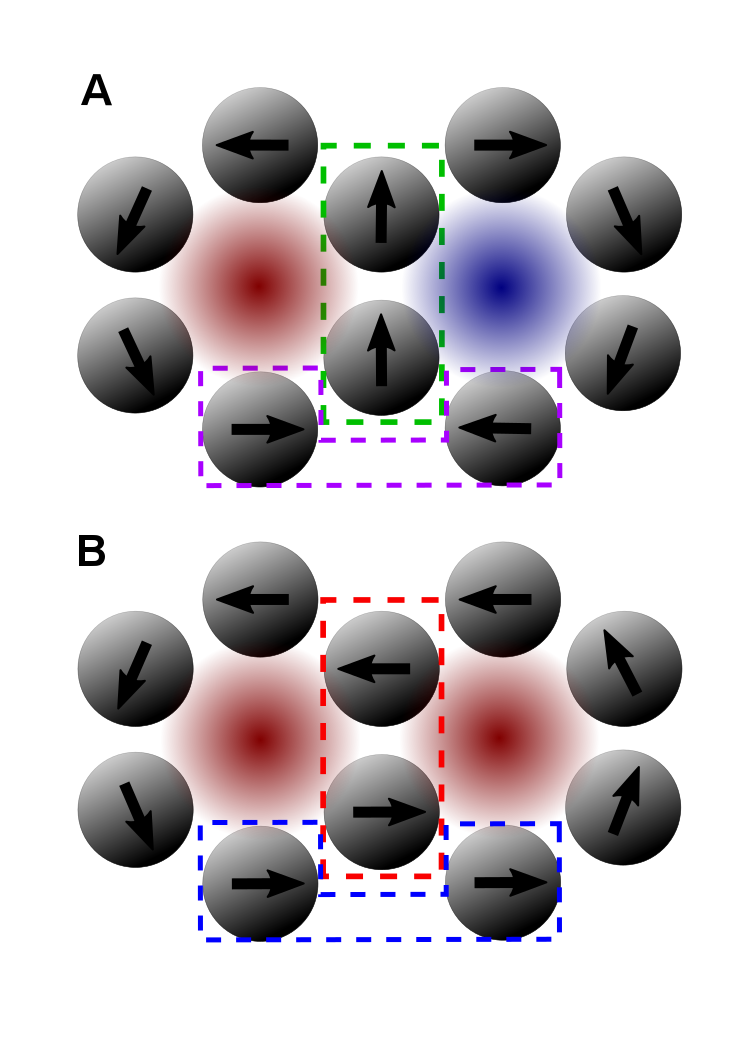
\includegraphics[trim = 0.5in 0.5in 0.5in 0.5in,clip=true,scale=0.4]{nn-ns-boxes_3.png}
  \caption{The NS (A) and NN (B) modes of the magnetic dimer system, including dipole arrangements in each mode. The green (NS) and red (NN) boxes highlight the interactions between the center two nanoparticles. In the NS mode, the dipoles are in a collinear arrangement, which is energetically favorable over the anti-parallel arrangement of the NN mode. The purple (NS) and blue (NN) boxes show some of the long-distance interactions. The purple box contains an anti-collinear arrangement of dipoles, which is more energetically unfavorable than the collinear arrangement contained within the blue box. Overall the long-distance interactions in the NN mode appear to be more favorable than the long-distance interactions in the NS mode. The red glow indicates a ``north'' magnetic moment, and the blue glow indicates a ``south'' magnetic moment.}
  \label{fig3}
  \end{center}
\end{figure}

The fully retarded electric field is composed of three parts: the near-field term (Equation 2), the intermediate-field term (Equation 3), and the far-field term (Equation 4). The intermediate-field term contributes the same energy ordering as the near-field term: collinear dipoles are favored more than anti-parallel dipoles. The far-field term, however, is energetically unfavorable for anti-parallel interactions and energetically preferable for parallel interactions. These three terms account for all of the retardation effects\cite{Purcell1973}.

\begin{figure}
  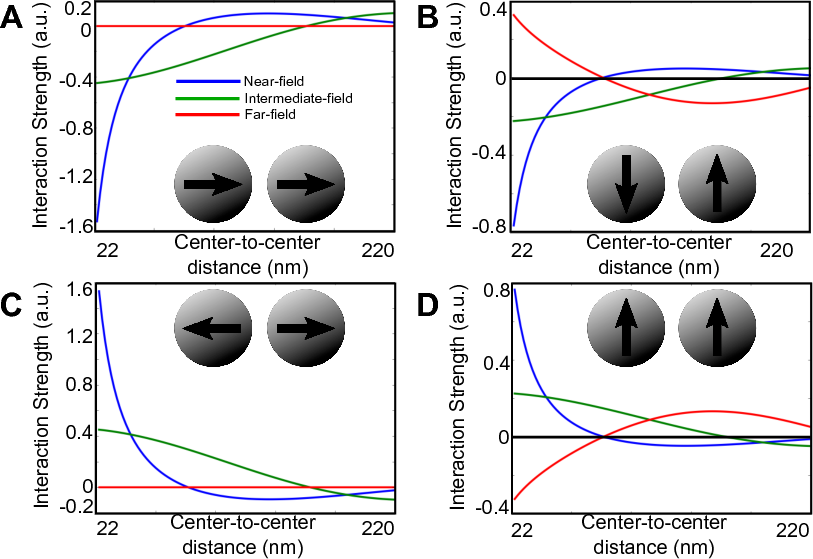
\includegraphics[scale=0.5]{dimer_interaction_3.png}
  \caption{Breakdown of the distance dependence of the fully retarded electric field for various dipole arrangements. A) At short range, collinear dipoles are energetically favorable in the near- and intermediate-field terms. There is long-distance regime in which collinear dipoles are unfavorable at around 150 nm. The far-field does not contribute. B) Anti-parallel dipoles are preferred in the near- and intermediate-field but are not in the far-field at short ditances. At longer distances (80-120 nm), the far-field term causes anti-parallel dipoles to become energetically favorable. C) The anti-collinear dipoles exhibit the opposite behavior of the collinear dipoles, becoming enegetically favorable at longer distances. D) The parallel dipoles exhibit the opposite behavior of the unfavorable at long distances. For large systems, the expected energy-ordering of ``bonding'' and ``anti-bonding'' hybridized modes in the quasistatic limit is not replicated by the fully retarded interaction. }
  \label{fig4}
\end{figure}

To understand the contributions to dipole-dipole coupling of each part of the fully retarded electric field, the interaction strengths for each term were computed for four planar hybridized modes of a silver nanosphere dimer. The results of these computations are displayed in Figure~\ref{fig4} and show how the interaction terms behave in various size regimes. The most obvious trait to note is that the far-field term is zero for both collinear and anti-collinear arrangements of dipoles. Second, the collinear and anti-collinear interactions are exact opposites of each other, with the same being true for the parallel and anti-parallel arrangements, as these represent equal and opposite interactions. Third the interaction strengths have slow oscillatory behavior over long length scales. Fourth, and perhaps most importantly, there are distinct distance regimes in which each term is more energetically favorable than the others. This final observation lends credence to the idea that the long-distance interactions in the NN mode are more favorable than those in the NS mode.

Incorporating the fully retarded electric field, the inter-particle coupling is no longer approximately a nearest-neighbor interaction, but rather a short- and long-distance coupling that accounts for the interactions among all particles. As the system grows larger, intermediate- and far-field interactions become stronger in proportion to the dominant near-field interactions. In the purple box of Figure~\ref{fig3}A, the dipoles are in an anti-collinear, anti-bonding arrangement: an energetically unfavorable interaction in both the near- and intermediate-field terms. Conversely, the dipole arrangement in the blue box of Figure~\ref{fig3}B is a collinear, bonding interaction, which is energetically preferred. Additionally, observing all of the complementary dipoles around the two ring system for both modes, it can be seen that the long-distance interactions in the NN mode are energetically favorable, and the long-distance interactions in the NS mode are energetically unfavorable. In the quasistatic limit, these interactions are weak, but when the intermediate- and far-field contributions are included, these interactions contribute to the total energy of each mode and the NN mode becomes energetically preferred over the NS mode at large enough sizes.

Returning to the tight-binding model, retardation effects are included by using the full interaction term in the Hamiltonian. The interaction terms depend on $\omega$, the frequency at which the collective mode resonates. This means that the Hamiltonian must now be diagonalized iteratively, beginning by using the LSPR frequency $\omega_{sp}$ of a sphere and resubstituting the resonant frequency of the mode of interest until the value converges. Additionally, the contribution of radiation damping\cite{vonPlessen2007} is introduced by adding a term to the bulk damping coefficient proportional to $\tau=\frac{2e^2}{3m_{sp}c^3}$ which causes a slight redshift in the LSPR frequency. Figure~\ref{fig5} tracks the eigenvalues of the NN and NS mode as a function of radius using the full Hamiltonian. The nanoparticle radius ranges from 1 nm to 20 nm, and the center-to-center distance between nanoparticles is always $2.2 \, r_0$, as in the diagram in Figure~\ref{fig1}. Below 10 nm, NS is the lowest-energy mode. Between 10 and 11 nm, the eigenvalues cross, and from 11 nm onward NN is the lowest-energy mode.

\begin{figure}
  \begin{center}
  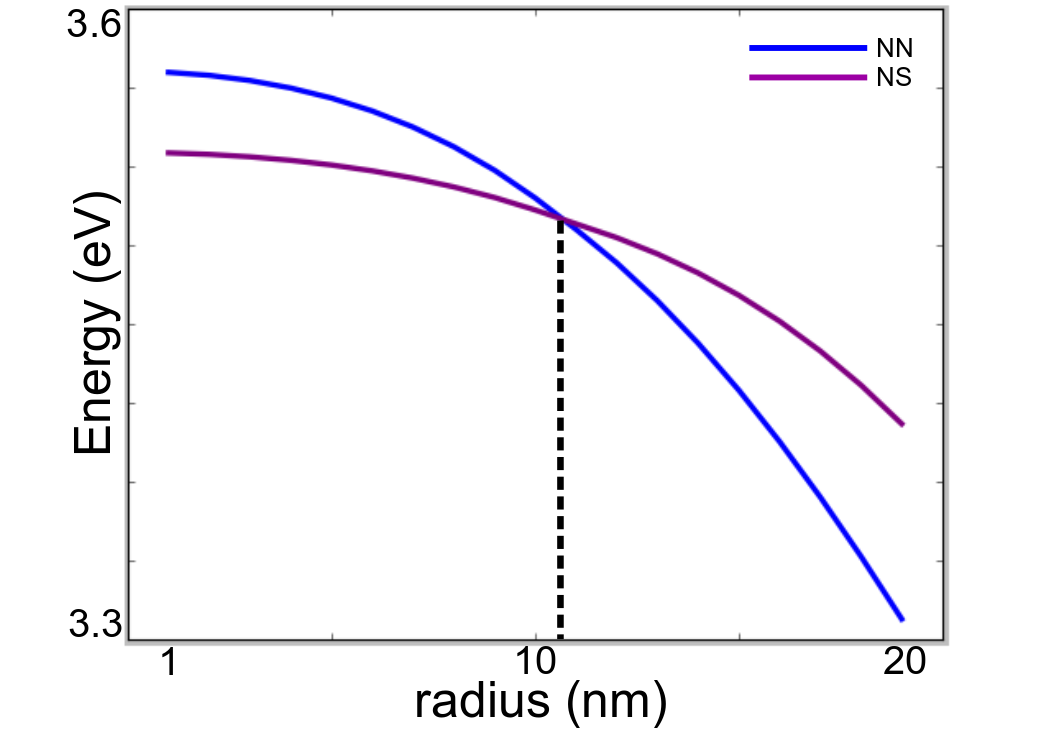
\includegraphics[trim= 0 0 0 0,clip=true,scale=0.3]{nn-ns-eigen_3.png}
  \caption{The eigenenergies of the NS and NN modes are tracked as a function of increasing radius. The critical radius is between 10 and 11 nm, where the NN mode becomes energetically preferential to the NS mode.}
  \label{fig5}
  \end{center}
\end{figure}

This is further verified by full-wave electrodynamics simulations\cite{Hohenester2012}. EELS simulations on magnetic dimer systems of different sizes show that in the quasistatic limit the NN mode is always higher in energy than the NS mode. Conversely, fully retarded simulations show that the NN mode eventually redshifts past the NS mode with increasing dimer size. Because the NS and NN modes are energetically nearly degenerate and their linewidths are broad, a Drude model for silver with a reduced damping coefficient was used as the dielectric function for the spheres. Running simulations for sphere radii between 1 nm and 10 nm and separation distances of $2.2 \, r_0$, it is found that the NN mode redshifts past the NS mode between 5 and 10 nm. The simulated EEL spectra are presented in Figure~\ref{fig6}. In the quasistatic limit, just as predicted, the modes did not change in energy with increasing particle size, due to the fact that the separation distances are parameterized by the radius. The interaction energy scales as $\frac{1}{r_{0}^{3}}$ and the polarizability scales as $r_{0}^{3}$, so these effects directly cancel and the modes do not change with increasing particle size in the quasistatic limit.

\begin{figure}
  \begin{center}
  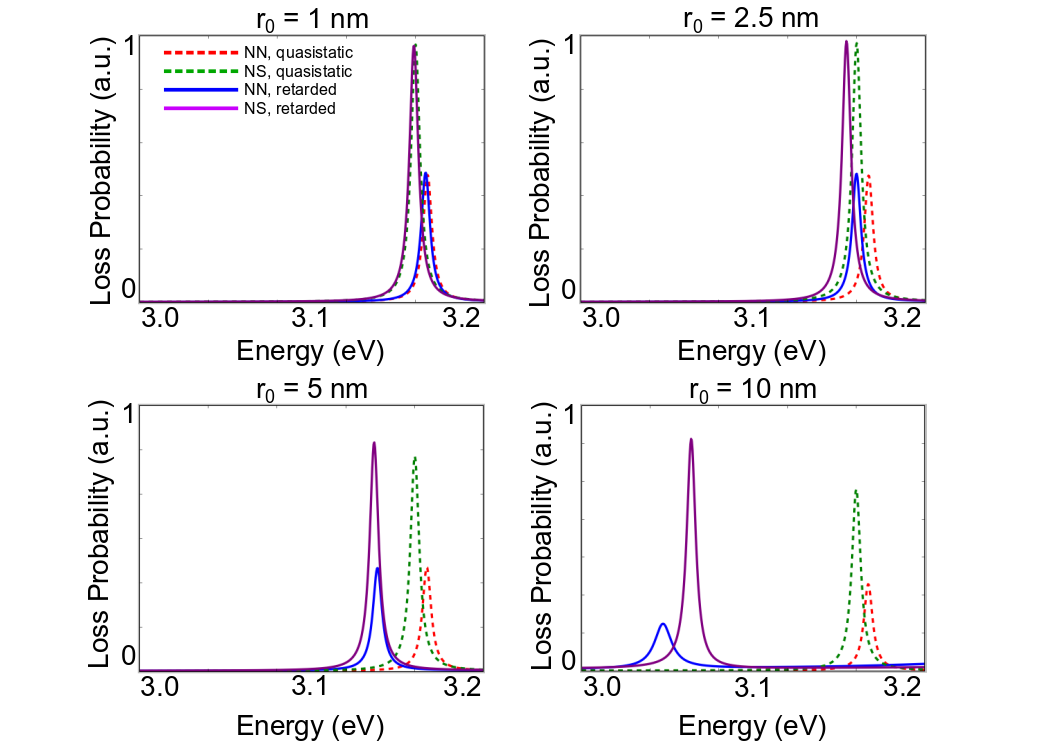
\includegraphics[trim = 0.8in 0 1.2in 0,clip=true,scale=0.5]{bem_spectra_3.png}
  \caption{Simulated quasistatic and fully retarded EEL spectra for the magnetic dimer with $r_0$ = 1 nm, 2.5 nm, 5 nm, and 10 nm. When the particles are very small, the quasistatic NS (green) and NN (red) modes are nearly energetically degenerate with the fully retarded NS (purple) and NN (blue) modes. As the size increases, the red and green traces do not move, but the purple and blue traces begin to redshift. Between 5 and 10 nm, the blue trace redshifts past the purple trace, indicating that in this size regime the NN mode is energetically favorable.}
  \label{fig6}
  \end{center}
\end{figure}

It has been shown that for small magnetic oligomer systems, specifically naphthalene-like decamers of silver nanospheres, quasistatic plasmon hybridization theory and fully retarded, full-wave numerical simulations agree on the energy-ordering of the magnetic modes. However, as the individual nanoparticles become larger and proportionally farther apart, the quasistatic limit breaks down and the simulations predict a different energy-ordering than the tight-binding model. Introducing retardation effects into the tight-binding model requires including the time-dependence of the near-field as well as the entire intermediate- and far-field terms. Consideration of these retardation effects also introduces radiation damping, which further impacts the resonant frequencies and broadening of the collective modes. Implementing this and iteratively solving for the eigenvalues of the collective magnetic modes, it is shown that including the fully retarded electric field properly predicts the energy-ordering in agreement with simulation. This gives a new route to the qualitative characterization of large, multi-constituent nanoparticle aggregates and accurately predicting the energy-ordering of the collective modes in various size regimes.

%%%%%%%%%%%%%%%%%%%%%%%%%%%%%%%%%%%%%%%%%%%%%%%%%%%%%%%%%%%%%%%%%%%%%
%% The ``Acknowledgement'' section can be given in all manuscript
%% classes.  This should be given within the ``acknowledgement''
%% environment, which will make the correct section or running title.
%%%%%%%%%%%%%%%%%%%%%%%%%%%%%%%%%%%%%%%%%%%%%%%%%%%%%%%%%%%%%%%%%%%%%
\begin{acknowledgement}
Thanks mom and dad, also whoever paid us. Thanks Masiello group for being cool. Thanks for not barfing after you read this. And thanks Hillary Clinton for being my idol.
\end{acknowledgement}

%%%%%%%%%%%%%%%%%%%%%%%%%%%%%%%%%%%%%%%%%%%%%%%%%%%%%%%%%%%%%%%%%%%%%
%% The appropriate \bibliography command should be placed here.
%% Notice that the class file automatically sets \bibliographystyle
%% and also names the section correctly.
%%%%%%%%%%%%%%%%%%%%%%%%%%%%%%%%%%%%%%%%%%%%%%%%%%%%%%%%%%%%%%%%%%%%%
\bibliography{references}
\end{document}
